\documentclass{beamer}
\usetheme{tokitex}

\usepackage{tikz}
\usepackage{graphics}
\usepackage{multirow}
\usepackage{tabto}
\usepackage{xspace}
\usepackage{amsmath}
\usepackage{hyperref}
\usepackage{wrapfig}
\usepackage{mathtools}

\usepackage{tikz}
\usepackage{clrscode3e}
\usepackage{gensymb}

\usepackage[english,bahasa]{babel}
\newtranslation[to=bahasa]{Section}{Bagian}
\newtranslation[to=bahasa]{Subsection}{Subbagian}

\usepackage{listings, lstautogobble}
\usepackage{color}

\definecolor{dkgreen}{rgb}{0,0.6,0}
\definecolor{gray}{rgb}{0.5,0.5,0.5}
\definecolor{mauve}{rgb}{0.58,0,0.82}

\lstset{frame=tb,
  language=c++,
  aboveskip=0mm,
  belowskip=0mm,
  showstringspaces=false,
  columns=fullflexible,
  keepspaces=true,
  basicstyle={\small\ttfamily},
  numbers=none,
  numberstyle=\tiny\color{gray},
  keywordstyle=\color{blue},
  commentstyle=\color{dkgreen},
  stringstyle=\color{mauve},
  breaklines=true,
  breakatwhitespace=true,
  lineskip={-3pt}
}

\usepackage{caption}
\captionsetup[figure]{labelformat=empty}

\newcommand{\progTerm}[1]{\textbf{#1}}
\newcommand{\foreignTerm}[1]{\textit{#1}}
\newcommand{\newTerm}[1]{\alert{\textbf{#1}}}
\newcommand{\emp}[1]{\alert{#1}}
\newcommand{\statement}[1]{"#1"}

\newcommand{\floor}[1]{\lfloor #1 \rfloor}
\newcommand{\ceil}[1]{\lceil #1 \rceil}
\newcommand{\abs}[1]{\left\lvert#1\right\rvert}
\newcommand{\norm}[1]{\left\lVert#1\right\rVert}

% Getting tired of writing \foreignTerm all the time
\newcommand{\farray}{\foreignTerm{array}\xspace}
\newcommand{\fArray}{\foreignTerm{Array}\xspace}
\newcommand{\foverhead}{\foreignTerm{overhead}\xspace}
\newcommand{\fOverhead}{\foreignTerm{Overhead}\xspace}
\newcommand{\fsubarray}{\foreignTerm{subarray}\xspace}
\newcommand{\fSubarray}{\foreignTerm{Subarray}\xspace}
\newcommand{\fbasecase}{\foreignTerm{base case}\xspace}
\newcommand{\fBasecase}{\foreignTerm{Base case}\xspace}
\newcommand{\ftopdown}{\foreignTerm{top-down}\xspace}
\newcommand{\fTopdown}{\foreignTerm{Top-down}\xspace}
\newcommand{\fbottomup}{\foreignTerm{bottom-up}\xspace}
\newcommand{\fBottomup}{\foreignTerm{Bottom-up}\xspace}
\newcommand{\fpruning}{\foreignTerm{pruning}\xspace}
\newcommand{\fPruning}{\foreignTerm{Pruning}\xspace}

\newcommand{\fgraph}{\foreignTerm{graph}\xspace}
\newcommand{\fGraph}{\foreignTerm{Graph}\xspace}
\newcommand{\froot}{\foreignTerm{root}\xspace}
\newcommand{\fRoot}{\foreignTerm{Root}\xspace}
\newcommand{\fnode}{\foreignTerm{node}\xspace}
\newcommand{\fNode}{\foreignTerm{Node}\xspace}
\newcommand{\fedge}{\foreignTerm{edge}\xspace}
\newcommand{\fEdge}{\foreignTerm{Edge}\xspace}
\newcommand{\fcycle}{\foreignTerm{cycle}\xspace}
\newcommand{\fCycle}{\foreignTerm{Cycle}\xspace}
\newcommand{\fdegree}{\foreignTerm{degree}\xspace}
\newcommand{\fDegree}{\foreignTerm{Degree}\xspace}
\newcommand{\fadjacencylist}{\foreignTerm{adjacency list}\xspace}
\newcommand{\fAdjacencylist}{\foreignTerm{Adjacency list}\xspace}
\newcommand{\fadjacencymatrix}{\foreignTerm{adjacency matrix}\xspace}
\newcommand{\fAdjacencymatrix}{\foreignTerm{Adjacency matrix}\xspace}
\newcommand{\fedgelist}{\foreignTerm{edge list}\xspace}
\newcommand{\fEdgelist}{\foreignTerm{Edge list}\xspace}
\newcommand{\flist}{\foreignTerm{list}\xspace}
\newcommand{\fList}{\foreignTerm{List}\xspace}
\newcommand{\fgraphtraversal}{\foreignTerm{graph traversal}\xspace}
\newcommand{\fGraphtraversal}{\foreignTerm{Graph traversal}\xspace}
\newcommand{\ftree}{\foreignTerm{tree}\xspace}
\newcommand{\fTree}{\foreignTerm{Tree}\xspace}
\newcommand{\fsubtree}{\foreignTerm{subtree}\xspace}
\newcommand{\fSubtree}{\foreignTerm{Subtree}\xspace}
\newcommand{\fparent}{\foreignTerm{parent}\xspace}
\newcommand{\fParent}{\foreignTerm{Parent}\xspace}
\newcommand{\fsibling}{\foreignTerm{sibling}\xspace}
\newcommand{\fSibling}{\foreignTerm{Sibling}\xspace}
\newcommand{\fpath}{\foreignTerm{path}\xspace}
\newcommand{\fPath}{\foreignTerm{Path}\xspace}
\newcommand{\fconnectedcomponent}{\foreignTerm{connected component}\xspace}
\newcommand{\fConnectedcomponent}{\foreignTerm{Connected component}\xspace}
\newcommand{\fbridge}{\foreignTerm{bridge}\xspace}
\newcommand{\fBridge}{\foreignTerm{Bridge}\xspace}
\newcommand{\farticulationpoint}{\foreignTerm{articulation point}\xspace}
\newcommand{\fArticulationpoint}{\foreignTerm{Articulation point}\xspace}
\newcommand{\ftreeedge}{\foreignTerm{tree edge}\xspace}
\newcommand{\fTreeedge}{\foreignTerm{Tree edge}\xspace}
\newcommand{\fbackedge}{\foreignTerm{back edge}\xspace}
\newcommand{\fBackedge}{\foreignTerm{Back edge}\xspace}
\newcommand{\fforwardedge}{\foreignTerm{forward edge}\xspace}
\newcommand{\fForwardedge}{\foreignTerm{Forward edge}\xspace}
\newcommand{\fcrossedge}{\foreignTerm{cross edge}\xspace}
\newcommand{\fCrossedge}{\foreignTerm{Cross edge}\xspace}
\newcommand{\fdiscoverytime}{\foreignTerm{discovery time}\xspace}
\newcommand{\fDiscoverytime}{\foreignTerm{Discovery time}\xspace}
\newcommand{\flowlink}{\foreignTerm{low link}\xspace}
\newcommand{\fLowlink}{\foreignTerm{Low link}\xspace}
\newcommand{\fstack}{\foreignTerm{stack}\xspace}
\newcommand{\fStack}{\foreignTerm{Stack}\xspace}
\newcommand{\for}{\foreignTerm{or}\xspace}
\newcommand{\fOr}{\foreignTerm{Or}\xspace}
\newcommand{\fand}{\foreignTerm{and}\xspace}
\newcommand{\fAnd}{\foreignTerm{And}\xspace}
\newcommand{\fcentroid}{\foreignTerm{centroid}\xspace}
\newcommand{\fCentroid}{\foreignTerm{Centroid}\xspace}

\newcommand{\fDivideAndConquer}{\foreignTerm{Divide and conquer}\xspace}
\newcommand{\fdivideAndConquer}{\foreignTerm{divide and conquer}\xspace}
\newcommand{\fMergeSort}{\foreignTerm{Merge sort}\xspace}
\newcommand{\fmergeSort}{\foreignTerm{merge sort}\xspace}
\newcommand{\fQuickSort}{\foreignTerm{Quicksort}\xspace}
\newcommand{\fquickSort}{\foreignTerm{quicksort}\xspace}
\newcommand{\fpivot}{\foreignTerm{pivot}\xspace}
\newcommand{\fPivot}{\foreignTerm{Pivot}\xspace}
\newcommand{\fbruteForce}{\foreignTerm{brute force}\xspace}
\newcommand{\fBruteForce}{\foreignTerm{Brute force}\xspace}
\newcommand{\fCompleteSearch}{\foreignTerm{complete search}\xspace}
\newcommand{\fExhaustiveSearch}{\foreignTerm{exhaustive search}\xspace}
\newcommand{\fbinarySearch}{\foreignTerm{binary search}\xspace}
\newcommand{\fBinarySearch}{\foreignTerm{Binary search}\xspace}
\newcommand{\fternarySearch}{\foreignTerm{ternary search}\xspace}
\newcommand{\fTernarySearch}{\foreignTerm{Ternary search}\xspace}
\newcommand{\funimodal}{\foreignTerm{unimodal}\xspace}
\newcommand{\fUnimodal}{\foreignTerm{Unimodal}\xspace}
\newcommand{\fGreedy}{\foreignTerm{Greedy}\xspace}
\newcommand{\fgreedy}{\foreignTerm{greedy}\xspace}
\newcommand{\fgreedyChoice}{\foreignTerm{greedy choice}\xspace}
\newcommand{\fGreedyChoice}{\foreignTerm{Greedy choice}\xspace}

\newcommand{\fdp}{\foreignTerm{dynamic programming}\xspace}
\newcommand{\fDp}{\foreignTerm{Dynamic programming}\xspace}
\newcommand{\fbitmask}{\foreignTerm{bitmask}\xspace}
\newcommand{\fBitmask}{\foreignTerm{Bitmask}\xspace}
\newcommand{\fstate}{\foreignTerm{state}\xspace}
\newcommand{\fState}{\foreignTerm{State}\xspace}
\newcommand{\fsubmask}{\foreignTerm{submask}\xspace}
\newcommand{\fSubmask}{\foreignTerm{Submask}\xspace}

\newcommand{\pheap}{\foreignTerm{heap}\xspace}
\newcommand{\pHeap}{\foreignTerm{Heap}\xspace}
\newcommand{\pBinaryHeap}{\foreignTerm{Binary Heap}\xspace}
\newcommand{\pbinaryHeap}{\foreignTerm{binary heap}\xspace}
\newcommand{\pHeapsort}{\foreignTerm{Heapsort}\xspace}
\newcommand{\pheapsort}{\foreignTerm{heapsort}\xspace}
\newcommand{\pdjs}{\foreignTerm{disjoint set}\xspace}
\newcommand{\pDjs}{\foreignTerm{Disjoint set}\xspace}

\newcommand{\fdotProduct}{\foreignTerm{dot product}\xspace}
\newcommand{\fDotProduct}{\foreignTerm{Dot product}\xspace}
\newcommand{\fcrossProduct}{\foreignTerm{cross product}\xspace}
\newcommand{\fCrossProduct}{\foreignTerm{Cross product}\xspace}
\newcommand{\fconvexHull}{\foreignTerm{convex hull}\xspace}
\newcommand{\fConvexHull}{\foreignTerm{Convex hull}\xspace}
\newcommand{\fgrahamScan}{\foreignTerm{graham scan}\xspace}
\newcommand{\fGrahamScan}{\foreignTerm{Graham scan}\xspace}
\newcommand{\flineSweep}{\foreignTerm{line sweep}\xspace}
\newcommand{\fLineSweep}{\foreignTerm{Line sweep}\xspace}

\newcommand{\fset}{\foreignTerm{set}\xspace}
\newcommand{\fSet}{\foreignTerm{Set}\xspace}
\newcommand{\fprefixSum}{\foreignTerm{prefix sum}\xspace}
\newcommand{\fPrefixSum}{\foreignTerm{Prefix sum}\xspace}
\newcommand{\ffenwickTree}{\foreignTerm{fenwick tree}\xspace}
\newcommand{\fFenwickTree}{\foreignTerm{Fenwick tree}\xspace}
\newcommand{\frangeSumQuery}{\foreignTerm{range sum query}\xspace}
\newcommand{\fRangeSumQuery}{\foreignTerm{Range sum query}\xspace}
\newcommand{\fquery}{\foreignTerm{query}\xspace}
\newcommand{\fQuery}{\foreignTerm{Query}\xspace}
\newcommand{\fsegmentTree}{\foreignTerm{segment tree}\xspace}
\newcommand{\fSegmentTree}{\foreignTerm{Segment tree}\xspace}
\newcommand{\fbinaryTree}{\foreignTerm{binary tree}\xspace}
\newcommand{\fBinaryTree}{\foreignTerm{Binary tree}\xspace}
\newcommand{\flazyPropagation}{\foreignTerm{lazy propagation}\xspace}
\newcommand{\fLazyPropagation}{\foreignTerm{Lazy propagation}\xspace}
\newcommand{\fsparseTable}{\foreignTerm{sparse table}\xspace}
\newcommand{\fSparseTable}{\foreignTerm{Sparse table}\xspace}

\newcommand{\ftrail}{\foreignTerm{trail}\xspace}
\newcommand{\fTrail}{\foreignTerm{Trail}\xspace}
\newcommand{\feulerTour}{\foreignTerm{euler tour}\xspace}
\newcommand{\fEulerTour}{\foreignTerm{Euler tour}\xspace}
\newcommand{\feulerTourTree}{\foreignTerm{euler tour tree}\xspace}
\newcommand{\fEulerTourTree}{\foreignTerm{Euler tour tree}\xspace}

\newcommand{\fmaxflow}{\foreignTerm{maximum flow}\xspace}
\newcommand{\fMaxflow}{\foreignTerm{Maximum flow}\xspace}
\newcommand{\fmincut}{\foreignTerm{minimum cut}\xspace}
\newcommand{\fMincut}{\foreignTerm{Minimum cut}\xspace}
\newcommand{\fflow}{\foreignTerm{flow}\xspace}
\newcommand{\fFlow}{\foreignTerm{Flow}\xspace}
\newcommand{\fsource}{\foreignTerm{source}\xspace}
\newcommand{\fSource}{\foreignTerm{Source}\xspace}
\newcommand{\fsink}{\foreignTerm{sink}\xspace}
\newcommand{\fSink}{\foreignTerm{Sink}\xspace}
\newcommand{\fbackEdge}{\foreignTerm{back-edge}\xspace}
\newcommand{\fBackEdge}{\foreignTerm{Back-edge}\xspace}
\newcommand{\fresidualCapacity}{\foreignTerm{residual capacity}\xspace}
\newcommand{\fResidualCapacity}{\foreignTerm{Residual capacity}\xspace}
\newcommand{\fbottleneck}{\foreignTerm{bottleneck}\xspace}
\newcommand{\fBottleneck}{\foreignTerm{Bottleneck}\xspace}
\newcommand{\faugmentingPath}{\foreignTerm{augmenting path}\xspace}
\newcommand{\fAugmentingPath}{\foreignTerm{Augmenting path}\xspace}


\title{Divide and Conquer}
\author{Tim Olimpiade Komputer Indonesia}
\date{}

\begin{document}

\begin{frame}
\titlepage
\end{frame}

\begin{frame}
\frametitle{Perkenalan}
\begin{itemize}
  \item Terkadang, permasalahan lebih mudah diselesaikan jika dibagi menjadi beberapa masalah yang lebih kecil.
  \item Masalah lebih kecil kemudian diselesaikan secara independen.
  \item Hasilnya digabungkan menjadi solusi untuk masalah yang lebih besar.
  \item Strategi ini digunakan Belanda pada masa penjajahan, biasa dipelajari pada sejarah sebagai \foreignTerm{devide et impera}.
\end{itemize}
\end{frame}

\begin{frame}
\frametitle{Konsep}
Secara umum, \newTerm{\fdivideAndConquer} terdiri dari tiga tahap:
\begin{itemize}
  \item \newTerm{divide}: membagi masalah yang besar menjadi masalah-masalah yang lebih kecil.
  \item \newTerm{conquer}: ketika sebuah masalah sudah cukup kecil untuk diselesaikan, langsung selesaikan.
  \item \newTerm{combine}: menggabungkan solusi dari masalah-masalah yang lebih kecil menjadi solusi untuk masalah yang besar.
\end{itemize}
\end{frame}

\begin{frame}
\frametitle{Ilustrasi Konsep}
\begin{figure}
  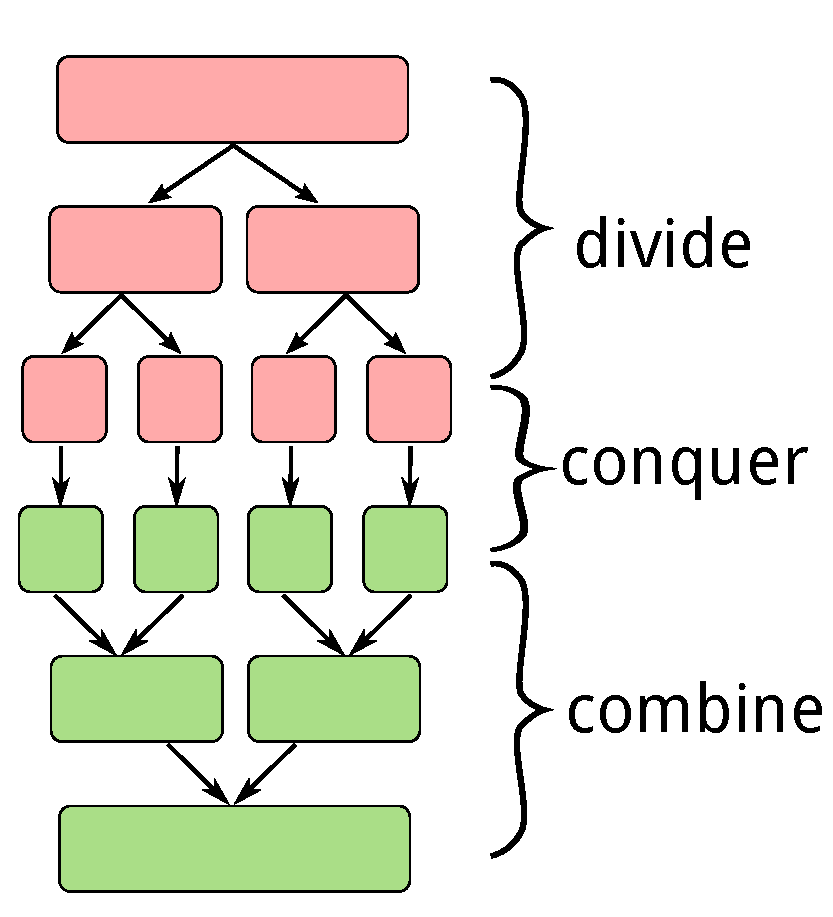
\includegraphics[width=6.5cm]{asset/dnc-concept.pdf}
\end{figure}
\end{frame}

\begin{frame}
\frametitle{Studi Kasus 1: Merge Sort}
\newTerm{\fMergeSort}: algoritma pengurutan O($N \log{N}$).
\newline
\newline
Prinsip kerja algoritma ini adalah:
\begin{itemize}
  \item \foreignTerm{divide}: jika \farray yang akan diurutkan berukuran besar, bagi menjadi dua \farray sama besar.
  \item \foreignTerm{conquer}: ketika \farray sudah cukup kecil untuk diurutkan, lakukan pengurutan.
  \item \foreignTerm{combine}: dari dua \farray yang telah terurut, gabungkan menjadi sebuah \farray terurut.
\end{itemize}
\end{frame}

\begin{frame}
\frametitle{Contoh Eksekusi Merge Sort}
Kapan suatu \farray dianggap cukup kecil untuk dapat diurutkan secara langsung?
\newline
\begin{itemize}
  \item Sederhana, yaitu ketika panjang \farray itu tinggal \emph{satu}.
  \item Tentu saja, \farray dengan panjang satu \emp{sudah pasti} terurut.
  \newline
\end{itemize}
Jadi selama \farray yang hendak diurutkan masih memiliki panjang lebih dari satu, bagi \farray itu menjadi dua.
\end{frame}

\begin{frame}
\frametitle{Contoh Eksekusi Merge Sort (lanj.)}
\fArray yang dimiliki masih terlalu besar, belah menjadi dua.
\begin{figure}
  \centering
  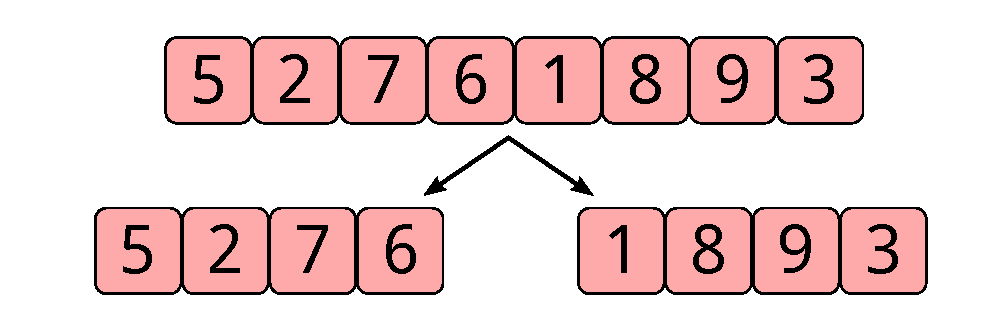
\includegraphics[width=10 cm]{asset/merge-sort-demo-1.pdf}
\end{figure}
\end{frame}

\begin{frame}
\frametitle{Contoh Eksekusi Merge Sort (lanj.)}
Masih belum cukup kecil, belah lagi.
\begin{figure}
  \centering
  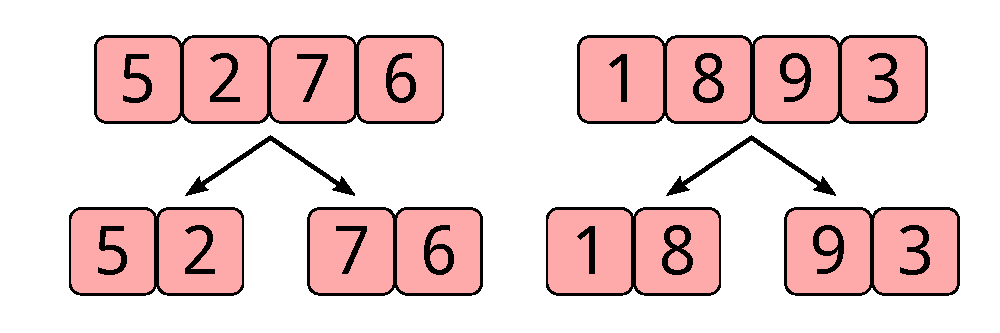
\includegraphics[width=10 cm]{asset/merge-sort-demo-2.pdf}
\end{figure}
\end{frame}

\begin{frame}
\frametitle{Contoh Eksekusi Merge Sort (lanj.)}
Masih belum cukup kecil, belah lagi.
\begin{figure}
  \centering
  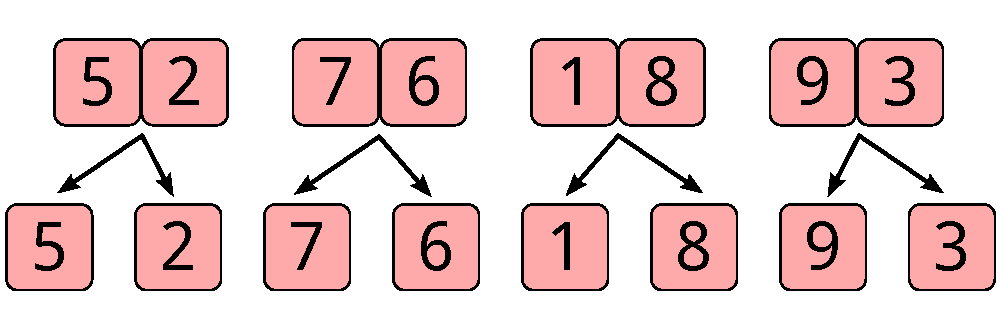
\includegraphics[width=10 cm]{asset/merge-sort-demo-3.pdf}
\end{figure}
\end{frame}

\begin{frame}
\frametitle{Contoh Eksekusi Merge Sort (lanj.)}
Kini kita memiliki \farray-\farray yang panjangnya hanya satu.\newline

Secara definisi, masing-masing \farray telah terurut.
\begin{figure}
  \centering
  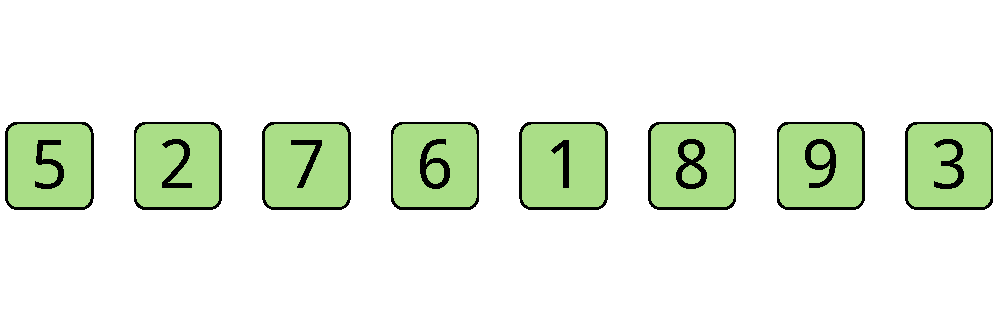
\includegraphics[width=10 cm]{asset/merge-sort-demo-4.pdf}
\end{figure}
\end{frame}

\begin{frame}
\frametitle{Contoh Eksekusi Merge Sort (lanj.)}
Gabungkan hasil pembelahan sebelumnya.
\begin{figure}
  \centering
  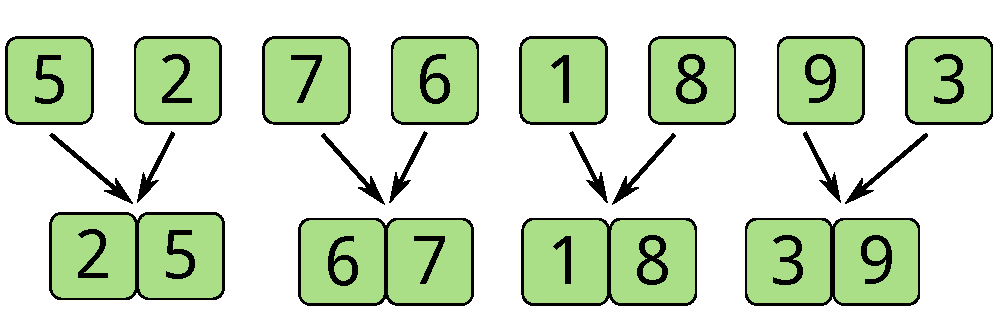
\includegraphics[width=10 cm]{asset/merge-sort-demo-5.pdf}
\end{figure}
\end{frame}

\begin{frame}
\frametitle{Contoh Eksekusi Merge Sort (lanj.)}
Gabungkan lagi.
\begin{figure}
  \centering
  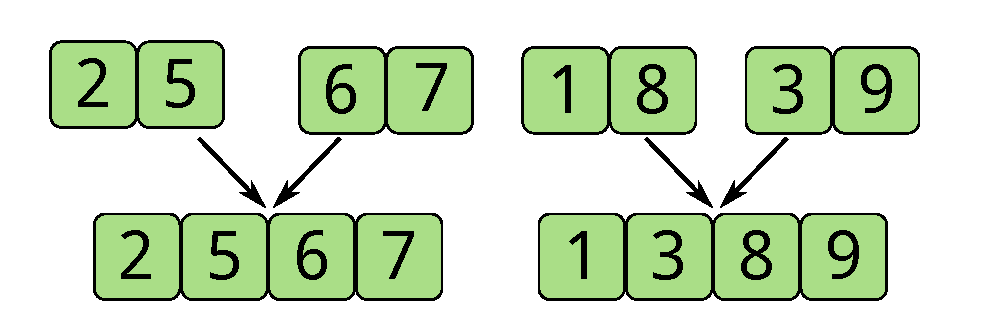
\includegraphics[width=10 cm]{asset/merge-sort-demo-6.pdf}
\end{figure}
\end{frame}

\begin{frame}
\frametitle{Contoh Eksekusi Merge Sort (lanj.)}
Gabungkan lagi dan akhirnya didapatkan \farray terurut.
\begin{figure}
  \centering
  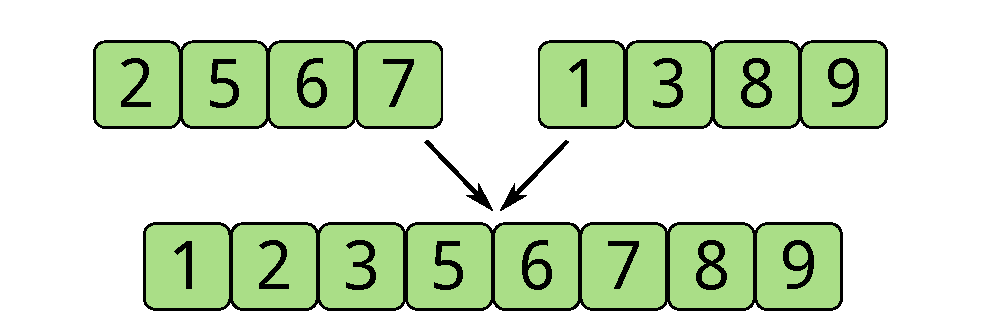
\includegraphics[width=10 cm]{asset/merge-sort-demo-7.pdf}
\end{figure}
\end{frame}

\begin{frame}
\frametitle{Menggabungkan Dua Array Terurut}
Bagaimana cara menggabungkan dua \farray yang telah terurut?
\begin{figure}
  \centering
  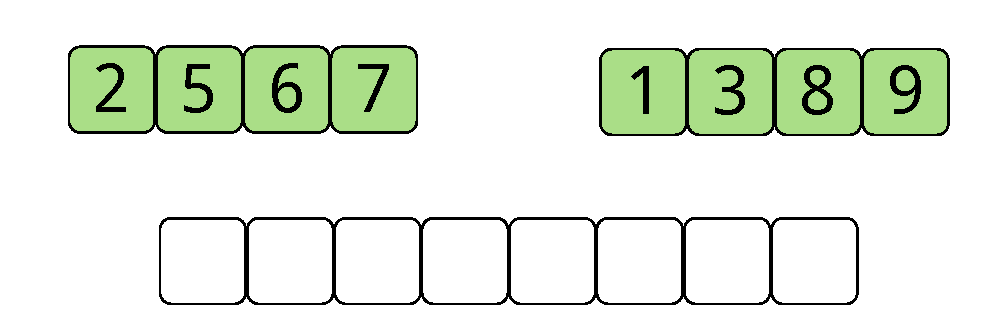
\includegraphics[width=10 cm]{asset/merge-array-pair-1.pdf}
\end{figure}
\end{frame}

\begin{frame}
\frametitle{Menggabungkan Dua Array Terurut (lanj.)}
Observasi: elemen terkecil dari \farray gabungan pasti salah satu dari elemen terkecil \farray yang terurut. Lebih tepatnya, yang memiliki nilai lebih kecil.
\begin{figure}
  \centering
  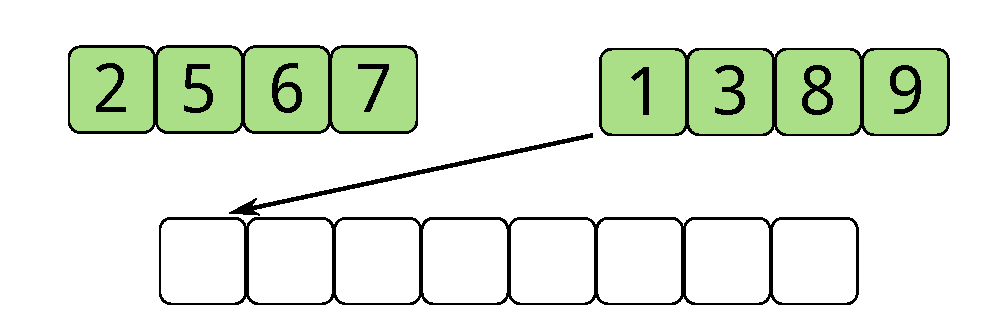
\includegraphics[width=10 cm]{asset/merge-array-pair-2.pdf}
\end{figure}
\end{frame}

\begin{frame}
\frametitle{Menggabungkan Dua Array Terurut (lanj.)}
Ulangi hal serupa sampai salah satu atau kedua \farray habis.

\begin{figure}
  \centering
  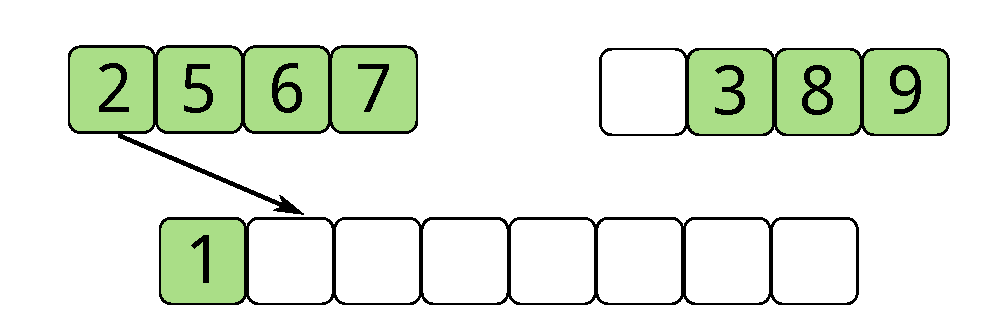
\includegraphics[width=10 cm]{asset/merge-array-pair-3.pdf}
\end{figure}
\end{frame}

\begin{frame}
\frametitle{Menggabungkan Dua Array Terurut (lanj.)}
\begin{figure}
  \centering
  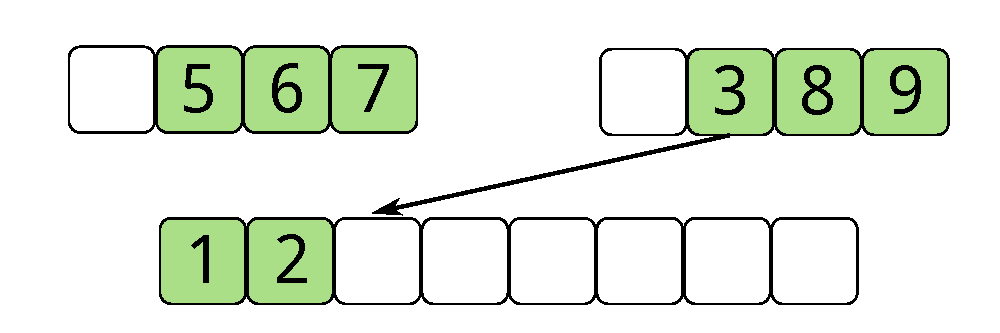
\includegraphics[width=10 cm]{asset/merge-array-pair-4.pdf}
\end{figure}
\end{frame}

\begin{frame}
\frametitle{Menggabungkan Dua Array Terurut (lanj.)}
\begin{figure}
  \centering
  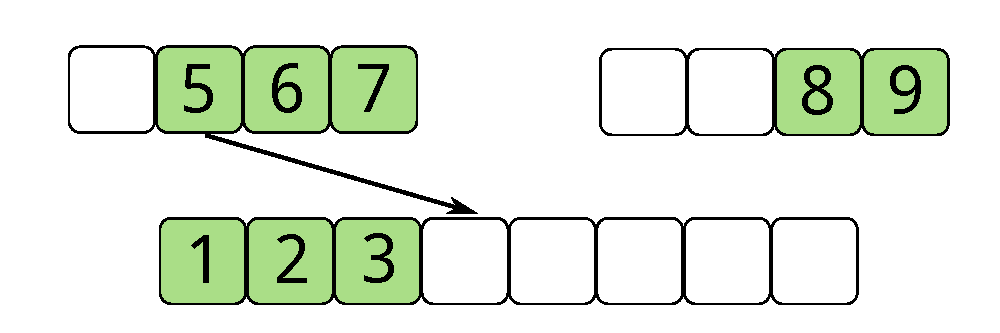
\includegraphics[width=10 cm]{asset/merge-array-pair-5.pdf}
\end{figure}
\end{frame}

\begin{frame}
\frametitle{Menggabungkan Dua Array Terurut (lanj.)}
\begin{figure}
  \centering
  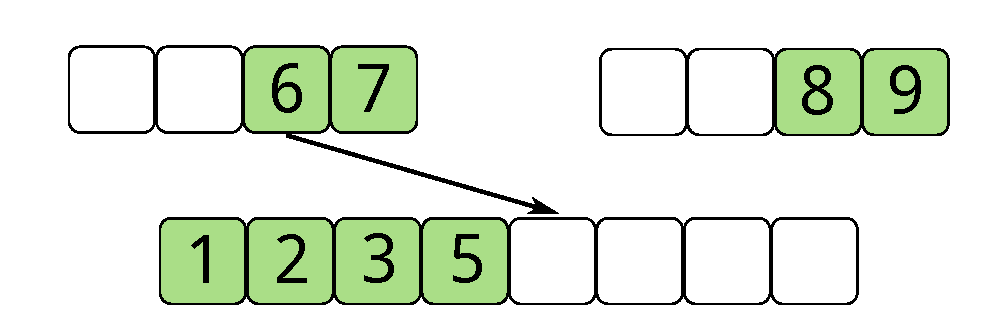
\includegraphics[width=10 cm]{asset/merge-array-pair-6.pdf}
\end{figure}
\end{frame}

\begin{frame}
\frametitle{Menggabungkan Dua Array Terurut (lanj.)}
\begin{figure}
  \centering
  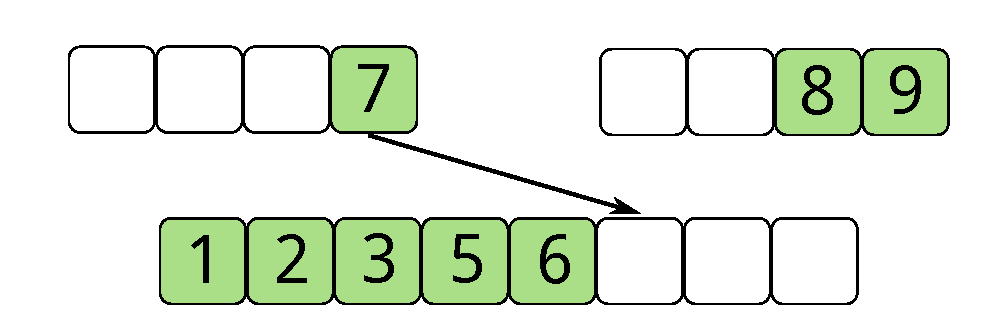
\includegraphics[width=10 cm]{asset/merge-array-pair-7.pdf}
\end{figure}
\end{frame}

\begin{frame}
\frametitle{Menggabungkan Dua Array Terurut (lanj.)}
Ketika salah satu \farray telah habis, \farray yang masih bersisa tinggal ditempelkan di akhir \farray gabungan.
\begin{figure}
  \centering
  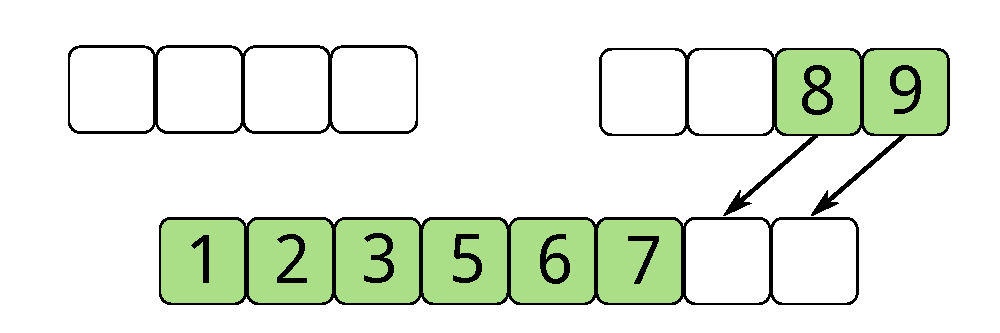
\includegraphics[width=10 cm]{asset/merge-array-pair-8.pdf}
\end{figure}
\end{frame}

\begin{frame}
\frametitle{Menggabungkan Dua Array Terurut (lanj.)}
Selesai proses menggabungkan.
\begin{figure}
  \centering
  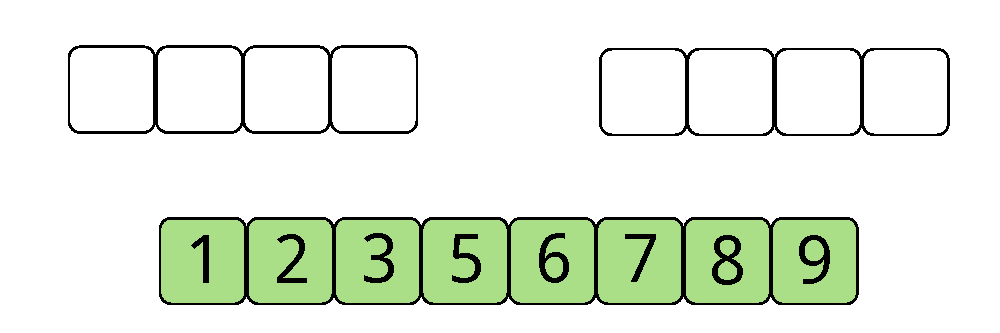
\includegraphics[width=10 cm]{asset/merge-array-pair-9.pdf}
\end{figure}
\end{frame}

\begin{frame}
\frametitle{Analisis Menggabungkan Dua Array Terurut}
\begin{itemize}
  \item Misalkan kedua \farray terurut yang akan digabung adalah $A$ dan $B$.
  \item Pada setiap langkah, salah satu dari elemen $A$ atau $B$ dipindahkan.
  \item Total terdapat $|A| + |B|$ proses, sehingga kompleksitasnya $O(|A| + |B|)$.
\end{itemize}
\end{frame}

\begin{frame}
\frametitle{Analisis Algoritma Merge Sort}
\begin{itemize}
  \item Misalkan $N$ menyatakan ukuran dari \farray.
  \item Dengan sifat membagi dua secara terus-menerus, kedalaman rekursif dari \fmergeSort adalah $O(\log{N})$
  \item Untuk setiap kedalaman, dilakukan aktivitas \foreignTerm{divide} dan \foreignTerm{combine}.
  \item Proses \foreignTerm{divide} dan proses \foreignTerm{conquer} selalu bekerja dalam $O(1)$.
\end{itemize}
\end{frame}

\begin{frame}
\frametitle{Analisis Algoritma Merge Sort (lanj.)}
\begin{figure}
  \centering
  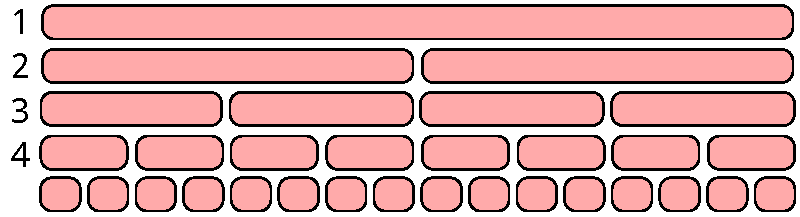
\includegraphics[width=10 cm]{asset/merge-sort-complexity.pdf}
\end{figure}
\begin{itemize}
  \item Kedalaman 1, proses \foreignTerm{combine} bekerja dalam $O(2 \times \frac{N}{2})$
  \item Kedalaman 2, proses \foreignTerm{combine} bekerja dalam $O(4 \times \frac{N}{4})$
  \item Kedalaman 3, proses \foreignTerm{combine} bekerja dalam $O(8 \times \frac{N}{8})$
  \item ...
\end{itemize}
\end{frame}

\begin{frame}
\frametitle{Analisis Algoritma Merge Sort (lanj.)}
\begin{itemize}
  \item Mudah untuk disadari bahwa keseluruhan proses untuk setiap kedalaman bekerja dalam $O(N)$.
  \item Karena kedalaman maksimal adalah $O(\log{N})$, kompleksitas akhir \fmergeSort adalah $O(N \log{N})$.
  \item Jauh lebih cepat dari algoritma pengurutan $O(N^2)$ seperti \foreignTerm{bubble sort}.
  \item \fMergeSort mampu mengurutkan \farray dengan ratusan ribu elemen dalam waktu singkat.
\end{itemize}
\end{frame}

%\begin{frame}
%\frametitle{Perbandingan Algoritma Pengurutan}
%TODO: grafik keren
%\end{frame}

\begin{frame}
\frametitle{Contoh Implementasi}
Mengurutkan $arr[left..right]$:
\noindent\rule{10cm}{0.4pt}
\begin{codebox}
\Procname{$\proc{mergeSort}(arr[], left, right)$}
\li \If $left \isequal right$ \Then
\li   \Comment Tinggal 1 elemen, sudah pasti terurut
\li \Else
\li   $mid \gets (left + right)$ div $2$
\li   $\proc{mergeSort}(arr, left, mid)$
\li   $\proc{mergeSort}(arr, mid+1, right)$
\li   $\proc{merge}(arr, left, mid, mid+1, right)$
    \End
\end{codebox}
\end{frame}

% WARNING: baris-baris ininn menggunakan perintah setcounter
% PASTIKAN ANDA MENGUBAHNYA JIKA ANDA MENGUBAH PSEUDOCODE
\begin{frame}
\frametitle{Contoh Implementasi (lanj.)}
Menggabungkan $arr[aLeft..aRight]$ dengan $arr[bLeft..bRight]$ yang telah terurut:
\noindent\rule{10cm}{0.4pt}
\begin{codebox}
\Procname{$\proc{merge}(arr[], aLeft, aRight, bLeft, bRight)$}
\li \Comment Buat array penampungan sementara bernama $temp$
\li \Comment Isikan $temp[aLeft \twodots bRight]$ dengan nilai dari $arr[aLeft \twodots bRight]$
\li $tIndex \gets 1$
\li $aIndex \gets aLeft$
\li $bIndex \gets bLeft$
\li $...$
\end{codebox}
\end{frame}

% WARNING: baris-baris ininn menggunakan perintah setcounter
% PASTIKAN ANDA MENGUBAHNYA JIKA ANDA MENGUBAH PSEUDOCODE
\begin{frame}
\frametitle{Contoh Implementasi (lanj.)}
\begin{codebox}
\setcounter{codelinenumber}{4}
\li $...$
\li \Comment Selama kedua \fsubarray masih ada isinya, ambil yang terkecil
\li \While $(aIndex \leq aRight)$ and $(bIndex \leq bRight)$ \Do
\li   \If $temp[aIndex] < temp[bIndex]$ \Then
\li     $arr[tIndex] \gets temp[aIndex]$
\li     $aIndex \gets aIndex + 1$
\li   \Else
\li     $arr[tIndex] \gets temp[bIndex]$
\li     $bIndex \gets bIndex + 1$
      \End
\li   $tIndex \gets tIndex + 1$
    \End
\li $...$
\end{codebox}
\end{frame}

% WARNING: baris-baris ininn menggunakan perintah setcounter
% PASTIKAN ANDA MENGUBAHNYA JIKA ANDA MENGUBAH PSEUDOCODE
\begin{frame}
\frametitle{Contoh Implementasi (lanj.)}
\begin{codebox}
\setcounter{codelinenumber}{13}
\li $...$
\li \Comment Masukkan \fsubarray yang masih bersisa
\li \Comment Hanya salah satu dari kedua while ini yang akan dieksekusi
\li \While $(aIndex \leq aRight)$ \Do
\li   $arr[tIndex] \gets temp[aIndex]$
\li   $aIndex \gets aIndex + 1$
\li   $tIndex \gets tIndex + 1$
    \End
\li \While $(bIndex \leq bRight)$ \Do
\li   $arr[tIndex] \gets temp[bIndex]$
\li   $bIndex \gets bIndex + 1$
\li   $tIndex \gets tIndex + 1$
    \End
\li \Comment selesai penggabungan
\end{codebox}
\end{frame}

\begin{frame}
\frametitle{Catatan Tentang Merge Sort}
\begin{itemize}
  \item \fMergeSort memiliki sifat \newTerm{\foreignTerm{stable}}.
  \item Artinya jika dua elemen $a_1$ dan $a_2$ memenuhi:
  \begin{itemize}
    \item memiliki yang nilai sama, dan
    \item sebelum diurutkan $a_1$ terletak sebelum $a_2$,
  \end{itemize}
  maka setelah diurutkan $a_1$ tetap terletak sebelum $a_2$.
\end{itemize}
\end{frame}

\begin{frame}
\frametitle{Studi Kasus 2: Mencari Nilai Terbesar}
\begin{itemize}
  \item Diberikan sebuah \farray $A$ yang memiliki $N$ bilangan.
  \item Cari nilai terbesar yang ada pada $A$!\newline
  \item Masalah ini mudah diselesaikan dengan perulangan biasa.
  \item Namun, coba kita selesaikan dengan \fdivideAndConquer.\end{itemize}
\end{frame}

\begin{frame}
\frametitle{Studi Kasus 2: Mencari Nilai Terbesar (lanj.)}
Pertama kita definisikan tahap-tahapnya:
\begin{itemize}
  \item \foreignTerm{Divide}: jika \farray berukuran besar, bagi menjadi dua \fsubarray.
  \item \foreignTerm{Conquer}: ketika \farray hanya berisi satu elemen, nilai terbesarnya pasti elemen tersebut.
  \item \foreignTerm{Combine}: nilai terbesar dari \farray adalah maksimum dari nilai terbesar di \fsubarray pertama dan nilai terbesar di \fsubarray kedua.
\end{itemize}
\end{frame}

\begin{frame}
\frametitle{Contoh Implementasi}
\begin{codebox}
\Procname{$\proc{findMax}(arr[], left, right)$}
\li \If $left \isequal right$ \Then
\li   \Return $arr[left]$
\li \Else
\li   $mid \gets (left + right)$ div $2$
\li   $leftMax \gets \proc{findMax}(arr, left, mid)$
\li   $rightMax \gets \proc{findMax}(arr, mid+1, right)$
\li   \Return $\func{max}(leftMax, rightMax)$
    \End
\end{codebox}
\end{frame}

\begin{frame}
\frametitle{Analisis Algoritma Mencari Nilai Terbesar}
\begin{figure}
  \centering
  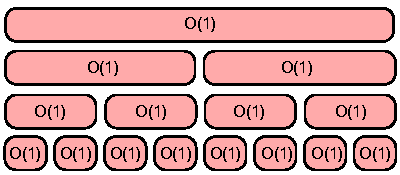
\includegraphics[width=8 cm]{asset/find-max-complexity.pdf}
\end{figure}
\begin{itemize}
  \item Setiap operasi \foreignTerm{divide}, \foreignTerm{conquer}, dan \foreignTerm{combine} bekerja dalam $O(1)$.
  \item Ketiga operasi tersebut dilaksanakan sebanyak\\1 + 2 + 4 + 8 + ... + $2^L$ kali, dengan $2^L$ mendekati $N$.
  \item Sehingga totalnya dilaksanakan sekitar $2^{L+1} - 1 = 2N$ operasi.
\end{itemize}
\end{frame}

\begin{frame}
\frametitle{Analisis Algoritma Mencari Nilai Terbesar (lanj.)}
\begin{itemize}
  \item Kompleksitas akhirnya adalah $O(N)$.
  \item Ternyata, strategi ini tidak lebih baik dari mencari nilai maksimum satu per satu.
  \item Kesimpulannya, \fdivideAndConquer \emp{tidak selalu} dapat mengurangi kompleksitas solusi naif.
\end{itemize}
\end{frame}

\begin{frame}
\frametitle{Penutup}
\begin{itemize}
  \item \fDivideAndConquer merupakan salah satu strategi dalam penyelesaian masalah.
  \item Konsep ini banyak digunakan pada struktur data lanjutan dan geometri komputasional.
  \item Jika suatu masalah dapat dibelah menjadi beberapa masalah yang lebih kecil dan serupa, kemudian hasil dari masing-masing penyelesaiannya dapat digabungkan, maka \fdivideAndConquer dapat digunakan.
\end{itemize}
\end{frame}

\end{document}
